\section{Component Design}

This section details the design of the components used in this project.

A very critical part of the design of a quadruped robot is the design of the mechanical legs. These legs must be able to handle the load of the robot and any other load that may be placed on it (referred to as static loads), along with withstanding the dynamic loads experienced when the robot is in motion. The design of mechanical legs involves choosing the actuator and its transmission mechanism, designing the structure of the mechanical leg, and choosing an efficient method of fabricating said mechanical leg.

The computing and control hardware also form a crucial part of the robot. The control hardware interfaces with the actuator and drives the actuator optimally to achieve the desired result. The control harware may use a lower level microcontroller to handle time-critical tasks such as leg actuator and dynamics control. A higher level computing unit may handle compute-intensive software and algorithms which are soft time-constrained, and also offer a user interface for intuitive control of the robot.

The power requirements of the actuators, compute, and control architectures also need to be met with high efficiency and with minimum weight, to minimize the dead weight of the robot and heat dissipation.


\newpage
\subsection{MG995 - Servo Motor}
MG995 is a servo motor that is popular for its acceptable performance and low price. The motor is used in many applications, including robotics and drones.The servo is suited for designing robotic arm in which wear and tear of motor is high. Being metal geared, the servo has long life and can be installed on system like robotic arm were motor work is huge.

MG995 has three terminals, as mentioned in pin diagram given in \ref{fig:MG995ServoPinout}. Pin function are given in \ref{table:MG995PinOut}.

\begin{table}[H]
\centering
    \begin{tabular}{ |c|c|c| } 
    \hline
    Pin & Name & Function\\
    \hline 
    1 & Signal pin (Orange pin) & Control PWM signal stating axis position\\
    2 & VCC (Red pin) & Input voltage from 5V - 7.2V power supply\\ 
    3 & Ground (Brown pin) & Ground terminal\\ 
    \hline
    \end{tabular}
    \caption{MG995 Servo Pinout}    
    \label{table:MG995PinOut}
\end{table}    
    
\begin{figure}[H]
    \centering
        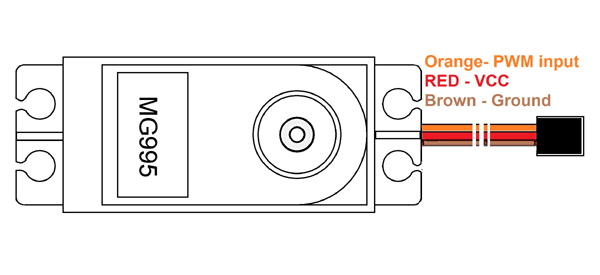
\includegraphics[width=0.35\textwidth]{MG995ServoPinout}
        \caption{MG995 Servo Pinout}
        \label{fig:MG995ServoPinout}
\end{figure}

\subsubsection{MG995 Features and Electrical characteristics}

\begin{itemize}
    \item Durable metal-geared servo
    \item Stable and shock proof double ball bearing design
    \item High speed rotation for quick response
    \item Fast control response
    \item Constant torque throughout the servo travel range
    \item Excellent holding power
    \item Weight: \(55 g\)
    \item Dimension: \(40.7 \times 19.7 \times 42.9mm\)
    \item Operating voltage range: \(4.8 V\) to \(7.2 V\) 
    \item Stall torque: \(9.4kg/cm \ (4.8v); 11kg/cm \ (6v)\)
    \item Operating speed: \(0.2s/60^o \ (4.8 V), \ 0.16s/60^o \ (6 V)\)
    \item Rotational degree: \(180^o\)
    \item Dead band width: \(5 \mu s\)
    \item Operating temperature range: \(0^oC \ to \ +55^oC\)
    \item Current draw at idle: \(10mA\)
    \item No load operating current draw: \(170mA\)
    \item Current at maximum load: \(1200mA\)
\end{itemize}

For controlling of servo there are only two important things to remember:

\begin{itemize}
    \item Frequency of PWM: The MG995 takes in PWM signals of frequency 50Hz; any higher or lower frequency PWM will lead to error. As shown in Figure \ref {fig:pwmPeriod} the every single cycle of PWM needs to be of 20ms width for 50Hz frequency.
    \item Duty cycle of PWM: The duty cycle of PWM (or ratio of ON time to total cycle time) determines the position of servo axis.
\end{itemize}

\begin{figure}[H]
    \centering
        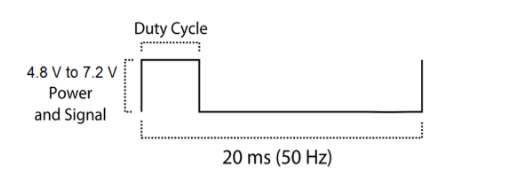
\includegraphics[width=0.5\textwidth]{pwmPeriod}
        \caption{PWM Period}
        \label{fig:pwmPeriod}
\end{figure}

\subsubsection{Schematic Diagram} 
%\ref{fig:mg2d}
\begin{figure}[H]
    \centering
        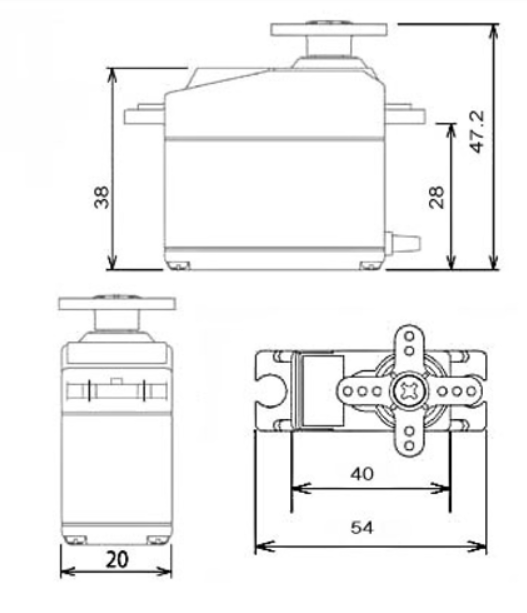
\includegraphics[width=0.5\textwidth]{mg2d}
        \caption{MG995 Schematic Diagram}
        \label{fig:mg2d}
\end{figure}


\newpage
\subsection{Raspberry Pi}
\subsubsection{Overview}

Raspberry Pi 4 Model B is the latest product in the popular Raspberry Pi range of computers. It offers ground-breaking increases in processor speed, multimedia performance, memory, and connectivity compared to the prior-generation Raspberry Pi 3 Model B+, while retaining backwards compatibility and similar power consumption. For the end user, Raspberry Pi 4 Model B (in Figure \ref{fig:raspi}) provides desktop performance comparable to entry-level x86 PC systems.

Key features include a high-performance 64-bit quad-core processor, dual-display support at resolutions up to 4K via a pair of micro-HDMI ports, hardware video decode at up to 4Kp60, up to 4GB of RAM, dual-band 2.4/5.0 GHz wireless LAN, Bluetooth 5.0, Gigabit Ethernet, USB 3.0, and PoE capability.

\begin{figure}[H]
    \centering
        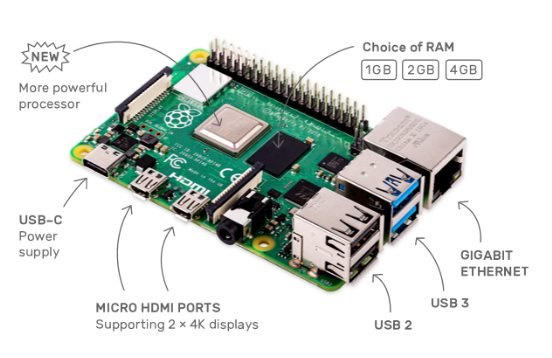
\includegraphics[width=0.75\textwidth]{raspi}
        \caption{Raspberry Pi 4B}
        \label{fig:raspi}
\end{figure}

\subsubsection{Specifications}
\begin{itemize}
    \item Processor: Broadcom BCM2711, quad-core Cortex-A72 (ARM v8) 64-bit SoC @ 1.5GHz
    \item Memory: 1GB, 2GB or 4GB LPDDR4 (depending on model)
    \item Connectivity: 2.4 GHz and 5.0 GHz IEEE 802.11b/g/n/ac wireless; Gigabit Ethernet; 2 \(\times\) USB 3.0 ports; 2 \(\times\) USB 2.0 ports 
    \item GPIO: Standard 40-pin GPIO header (fully backwards-compatible with previous boards)
    \item Video and sound: 2 \(\times\) micro HDMI ports (up to 4Kp60 supported); 2-lane MIPI DSI display port; 2-lane MIPI CSI camera port; 4-pole stereo audio and composite video port
    \item Multimedia: H.265 (4Kp60 decode); H.264 (1080p60 decode, 1080p30 encode); OpenGL ES, 3.0 graphics
    \item SD card support: Micro SD card slot for loading operating system and data storage
    \item Input power: 5V DC via USB-C connector (minimum 3A1); 5V DC via GPIO header (minimum 3A1); Power over Ethernet (PoE)-enabled (requires separate PoE HAT)
    \item Environment: Operating temperature \(0-50^oC\)
\end{itemize}
   
 
\newpage
\subsection{Arduino Mega}
\subsubsection{Overview}

The Arduino Mega 2560 is a microcontroller board based on the ATmega2560. It has 54 digital input/output pins (of which 15 can be used as PWM outputs), 16 analog inputs, 4 UARTs (hardware serial ports), a 16 MHz crystal oscillator, a USB connection, a power jack, an ICSP header, and a reset button. It contains everything needed to support the microcontroller; simply connect it to a computer with a USB cable or power it with a AC-to-DC adapter or battery to get started. The Mega 2560 board is compatible with most shields designed for the Uno and the former boards Duemilanove or Diecimila.

\begin{figure}[H]
    \centering
        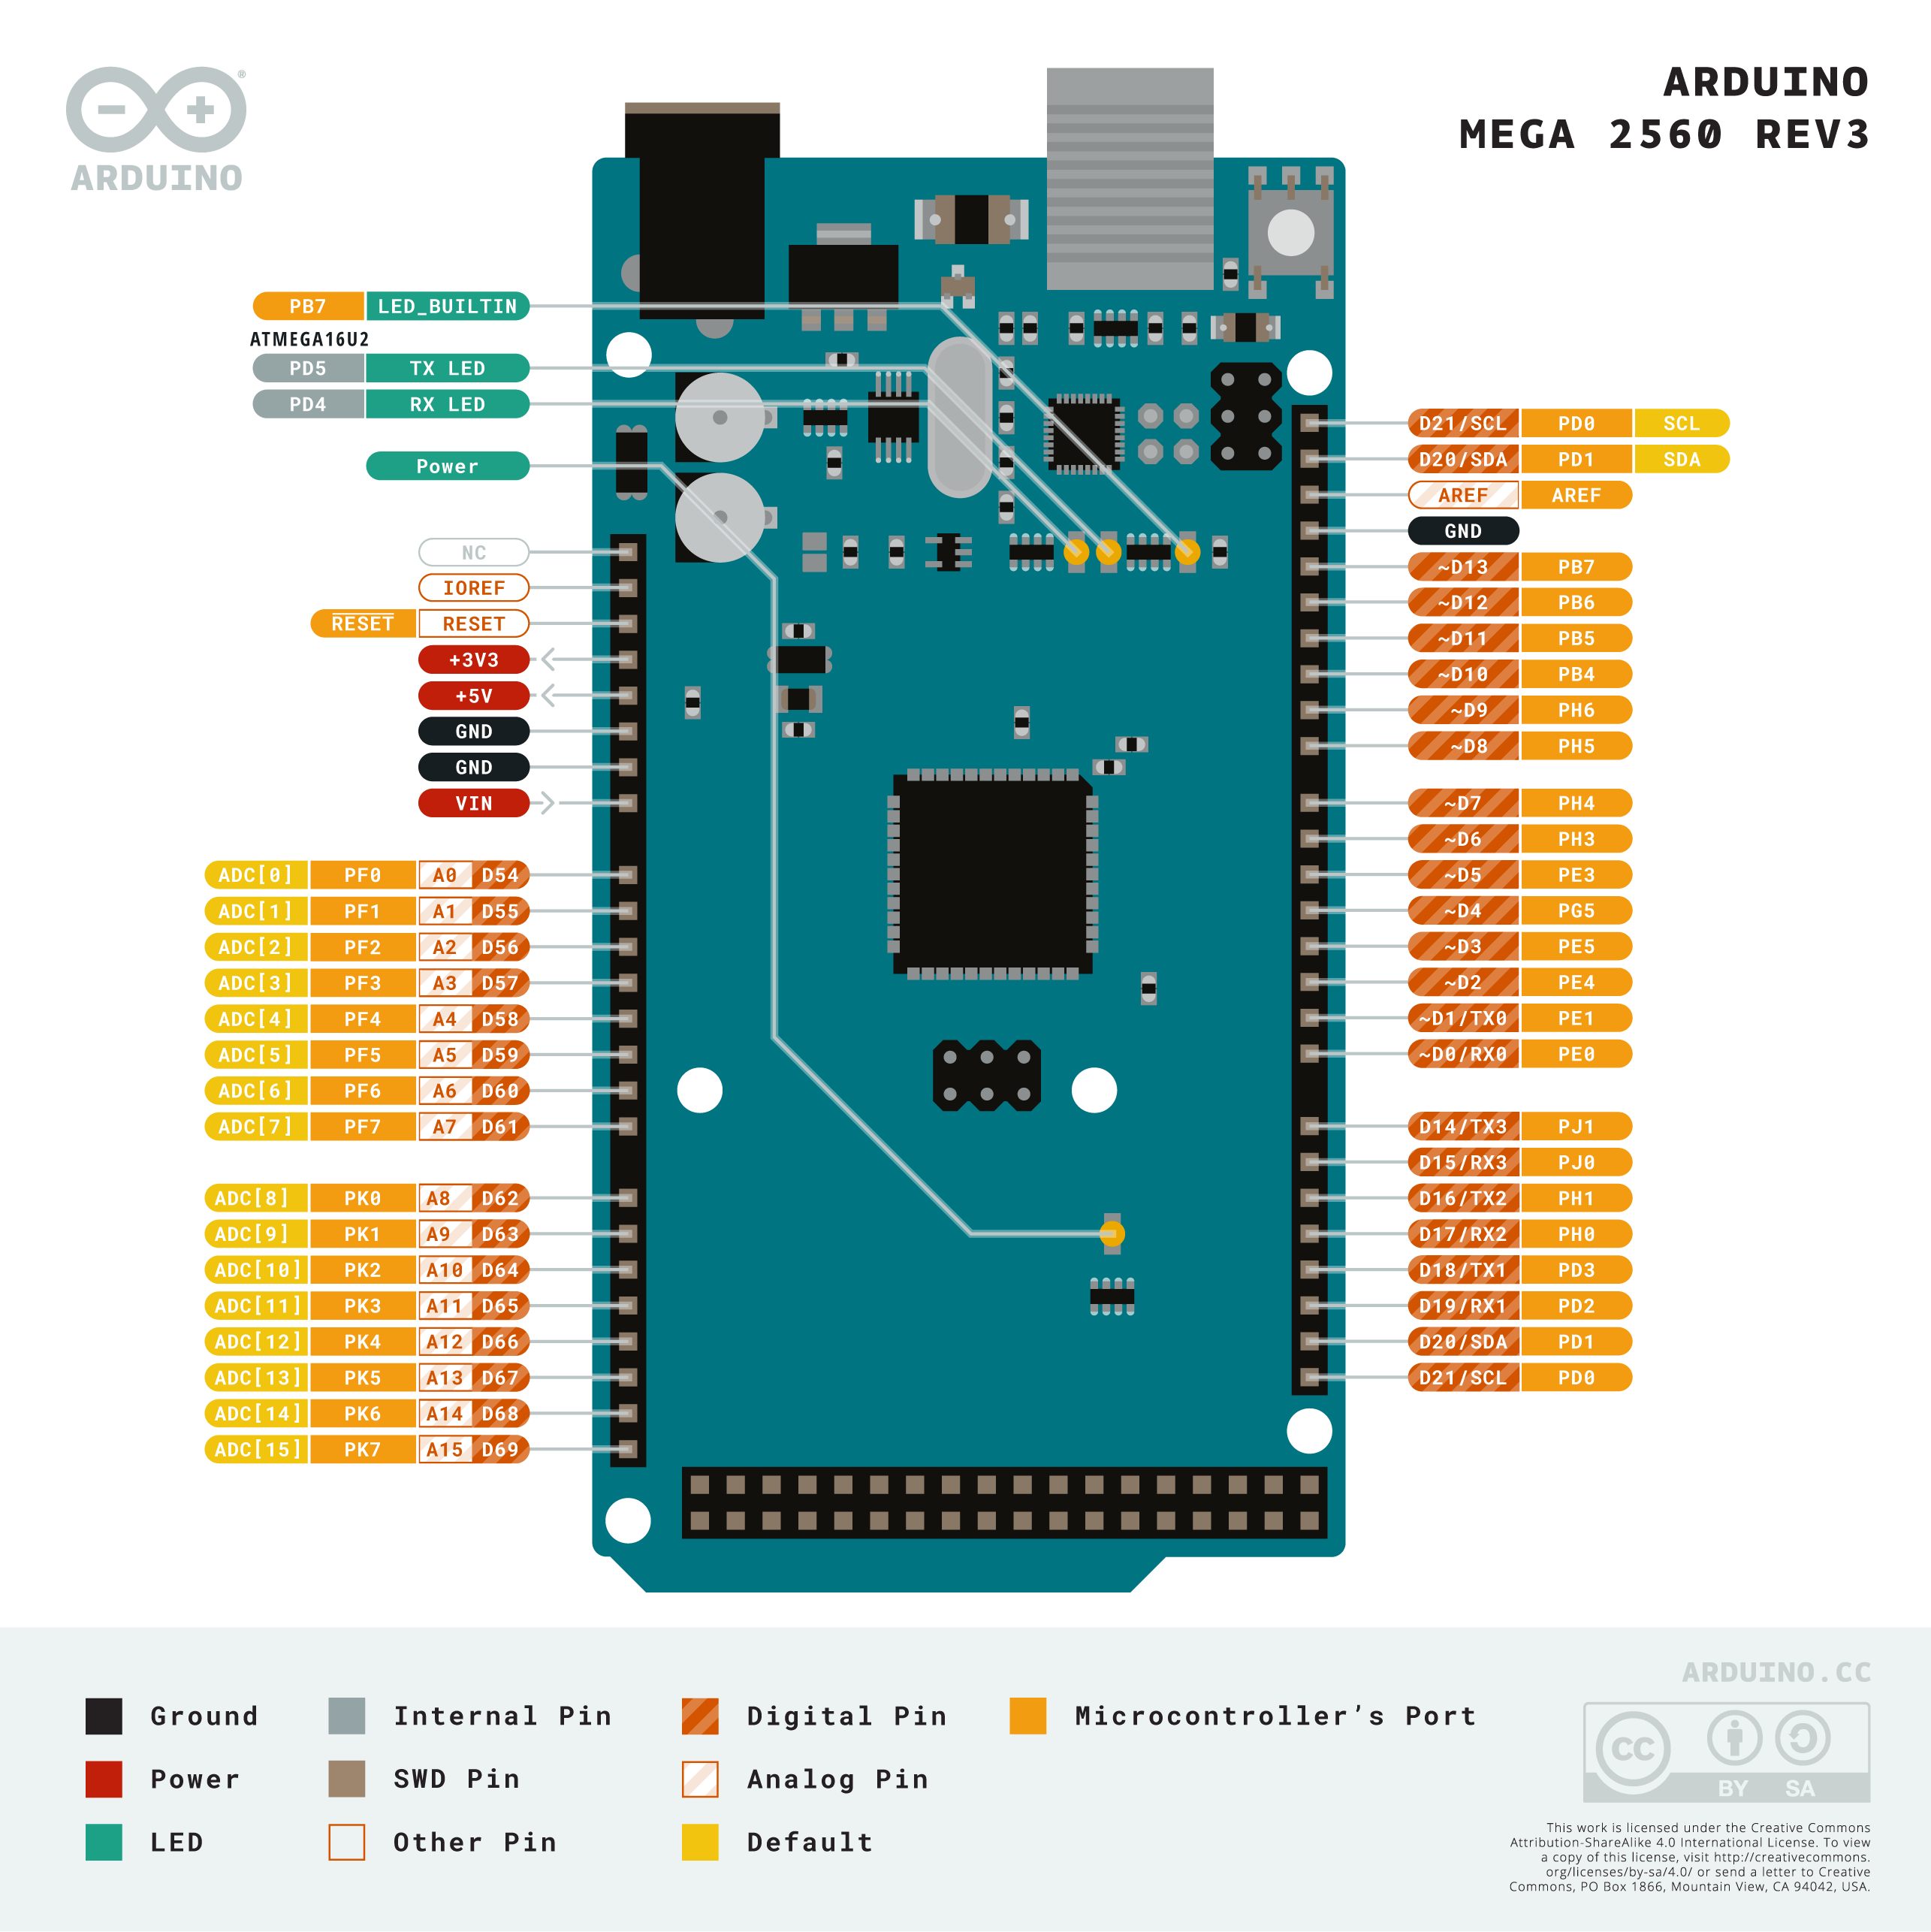
\includegraphics[width=0.55\textwidth]{megapinout}
        \caption{Ardunio Mega2560}
        \label{fig:megapinout}
\end{figure}

\newpage
\subsection{RPLiDAR A1M8}
\subsection{Stereo Camera}
\subsection{Ultrasonic Sensor}
\subsection{SMPS}

